\documentclass[a4paper,oneside]{report}
\usepackage{color}              %Farben, f.r \definecolor{}
\usepackage{amssymb}            %Mathematische Symbole
\usepackage{amsthm}             %Besseres \newtheorem
\usepackage{amsmath}            %Mathematische Umgebungen
\usepackage{mathtools}          %\xRightarrow, etc
\usepackage{mathrsfs}           %enthaelt \mathscr
\usepackage{graphicx}
\usepackage{enumerate}          % in-place numerations def.
\usepackage{fullpage}
\usepackage{array}
%\usepackage{multicol}
%\usepackage[notref,notcite]{showkeys}
%\usepackage{algorithm,algorithmic}
\usepackage{color}
\usepackage{graphicx}
\usepackage{xypic}
\entrymodifiers={+!!<0pt,\fontdimen22\textfont2>}
\usepackage[all]{xy}

%-----------------------------
%Hugrún's additions
\usepackage{hyperref}
\usepackage{blkarray}

\usepackage{tikz}
\newcommand{\LD}{\langle}
\newcommand{\RD}{\rangle}
\usepackage{tikz}
\usepackage{tikz,fullpage}
\usetikzlibrary{arrows,%
                petri,%
                topaths}%
\usepackage{tkz-berge}
\usepackage[position=top]{subfig}

%------------------------

\newtheoremstyle{myremark} % name
    {7pt}                    % Space above
    {7pt}                    % Space below
    {}  	                 % Body font
    {}                           % Indent amount
    {\bf}       	         % Theorem head font
    {.}                          % Punctuation after theorem head
    {.5em}                       % Space after theorem head
    {}  % Theorem head spec (can be left empty, meaning ‘normal’)

\theoremstyle{plain}
\newtheorem{lemma}{Lemma}
\newtheorem{theorem}[lemma]{Theorem}
\newtheorem{fact}[lemma]{Fact}
\newtheorem{definition}[lemma]{Definition}
\newtheorem{corollary}[lemma]{Corollary}
\newtheorem{proposition}[lemma]{Proposition}
\newtheorem{conjecture}[lemma]{Conjecture}
\newtheorem{observation}[lemma]{Observation}
\newtheorem{problem}[lemma]{Problem}
\newtheorem{notation}[lemma]{Notation}

\theoremstyle{myremark}
\newtheorem{remark}[lemma]{Remark}
\newtheorem{example}[lemma]{Example}

%-------------------------
% OUR MACROS
\newcommand{\compl}[1]{\overline{#1}}
\newcommand{\real}{\mathbb{R}}

%------------------------

\title{\bf Graph coloring}
\author{Micha{\l} Adamaszek \and ? \and ?}
%------------------------
\begin{document}

\maketitle
\tableofcontents

\chapter{Preface}

These lecture notes come from a master-level course \emph{Graph coloring}, taught by the first author at the University of Copenhagen in spring 2016.

Despite the name it is \emph{not} a comprehensive course in graph coloring. Instead, graph coloring problems serve only as a convenient excuse to familiarize the students, who may never have taken a more advanced combinatorics course, with interesting combinatorial techniques. The purpose is rather to give a taste of tools from linear algebra, calculus, combinatorics and geometry and demonstrate a few classical combinatorial theorems and their applications. It also has a bit of an experimental flavour and includes short programming exercises in Sage.

We are grateful for the contribution by the students who took notes during the course: Giorgia Laura Cassis, Hugr\'un Fj\'ola Hafsteinsd\'ottir, Rolf J{\o}rgensen, Mathis Elmgaard Isaksen, Sokratis Theodoridis, Mortan Janusarson Thomsen, Kristoffer Holm Nielsen.

The website for this course was \url{http://aszek.net/chromatic}. The LaTeX source of these lecture notes is available under the GNU GPL license from \url{http://github.com/aszek/chromatic}.
\chapter{Temporary}

\section{Notation}

A graph is $G=(V,E)$ and it has $n=|V|$, $m=|E|$. If there are more graphs the next one is $H$. A coloring with $c$ colors is a function $f:V\to \{1,\ldots,c\}=C$. The chromatic number is $\chi$. A bipartite graph has parts $A,B$, or $X,Y$.


\section{Aha foo bar}
This is just a testing ground for now.

Here is ade finition

\begin{definition} We say that a \emph{definition} is a definition is
\begin{equation}
\label{eq:def-eq-temp}
\int_M d\omega = \int_{\partial M} \omega
\end{equation}
\end{definition}

On the other hand, here is a remark:

\begin{remark}
I would like the contents of a remark not to be italicised.
\end{remark}

\section{Section}
It would be good to split each chapter into 2-4 sections.

\section{Including sage code}
We include SAGE source code like this:

\begin{verbatim}
def FunnyGraph(n):
    c = graphs.CompleteGraph(n)
    c.delete_edges(graphs.CycleGraph(n).edges())
    return graphs.MycielskiStep(c).join(graphs.WheelGraph(n+1))

G = FunnyGraph(99)
\end{verbatim}

At the very end I will implement it using a pygmentize highlighter for python.

Figures can be drawn in tikz or whatever, or included from another file. In any case, it would be good to have every figure inside a figure environment with a label and caption.

\section{TODOs}
List of todos for MA:
\begin{itemize}
\item Remove this file
\item Add pygmentize
\item Expand and check bibliography
\end{itemize}

\chapter{Basic graph theory}

Roughly lex1.tex and lec2.tex without defining chromatic number.

\chapter{Vertex coloring}

Define chromatic number and the lec3.tex, lec4.tex
\chapter{Planar graphs}

In this part we are going to focus on one of the most classical (and historical) topics in graph coloring: vertex colorings of planar graphs. 

\begin{definition}
$G$ is \emph{planar} if it can be drawn on ${\rm I\!R^2}$(the plane) so that edges intersect only at their common endpoints.
We call such a drawing an \emph{"embedding"}(some authors say \emph{"drawing"}).
\end{definition}

\begin{example}

\begin {tikzpicture}

\draw   
           node[fill,circle,inner sep=0pt,minimum size=3pt] (n1) at (0,0) {}
	node[fill,circle,inner sep=0pt,minimum size=3pt] (n2) at (1,0) {} 
	node[fill,circle,inner sep=0pt,minimum size=3pt] (n3) at (0,1) {} 
	node[fill,circle,inner sep=0pt,minimum size=3pt] (n4) at (1,1) {}
[line width = 1 pt, black, -] (n1) edge (n4)
[line width = 1 pt, black, -] (n2) edge (n3)
[line width = 1 pt, black, -] (n1) edge (n2)
[line width = 1 pt, black, -] (n2) edge (n4)
[line width = 1 pt, black, -] (n4) edge (n3)
[line width = 1 pt, black, -] (n3) edge (n1)
;
\end{tikzpicture}
       $K_4$ not an embedding
\begin {tikzpicture}
\newcommand*{\OutAngle}{60}
 \newcommand*{\ArcMax}{1.2}
\draw
	node[fill,circle,inner sep=0pt,minimum size=3pt] (n1) at (0,0) {}
	node[fill,circle,inner sep=0pt,minimum size=3pt] (n2) at (1,0) {} 
	node[fill,circle,inner sep=0pt,minimum size=3pt] (n3) at (0,1) {} 
	node[fill,circle,inner sep=0pt,minimum size=3pt] (n4) at (1,1) {}
[line width = 1 pt, black, -] (n1) edge (n2)
[line width = 1 pt, black, -] (n1) edge (n2)
[line width = 1 pt, black, -] (n2) edge (n4)
[line width = 1 pt, black, -] (n4) edge (n3)
[line width = 1 pt, black, -] (n3) edge (n1)
(0, 1) to[out=\OutAngle, in=135]
    (\ArcMax, \ArcMax) to[out=-45, in=90-\OutAngle]
    (1, 0) -- cycle
;
\end{tikzpicture}
embedding ($K_4$ is planar)
\newline
\newline
\begin {tikzpicture}
\draw 
%node[fill,circle,inner sep=0pt,minimum size=3pt] (n1) at (0,0) {}
node[fill,circle,inner sep=0pt,minimum size=3pt] (n2) at (-0.5,0) {}
node[fill,circle,inner sep=0pt,minimum size=3pt] (n3) at (0,0.5) {}
node[fill,circle,inner sep=0pt,minimum size=3pt] (n4) at (0.5,0) {}
node[fill,circle,inner sep=0pt,minimum size=3pt] (n5) at (0,1) {}
[line width = 1 pt, black, -] (n2) edge (n4)
%[line width = 1 pt, black, -] (n1) edge (n4)
[line width = 1 pt, black, -] (n3) edge (n5)
[line width = 1 pt, black, -] (n2) edge (n5)
[line width = 1 pt, black, -] (n4) edge (n5)
[line width = 1 pt, black, -] (n3) edge (n4)
[line width = 1 pt, black, -] (n2) edge (n3)
;
\end{tikzpicture}
straight line-embedding
\end{example}

\begin{theorem}(F{\'a}ry,\emph{1948}) If $G$ has an embedding, then it also has one where every edge is a straight line segment.
\end{theorem}
\begin{remark} $G$ can be treated as a topological space [($CW-$,$\Delta-$,simplicial-) complex]. Then $G$ is planar if (as a topological space) it embeds into ${\rm I\!R^2}$ ($embedding \equiv continuous, injective\ map$)
\end{remark}

\begin{example}
\begin {tikzpicture}
\draw  
	node[fill,circle,inner sep=0pt,minimum size=3pt] (n1) at (0,0) {}
	node[fill,circle,inner sep=0pt,minimum size=3pt] (n2) at (-1,0) {}
	node[fill,circle,inner sep=0pt,minimum size=3pt] (n3) at (1,0) {}
	node[fill,circle,inner sep=0pt,minimum size=3pt] (n4) at (0,-1) {}
	node[fill,circle,inner sep=0pt,minimum size=3pt] (n5) at (-1,-1) {}
	node[fill,circle,inner sep=0pt,minimum size=3pt] (n6) at (1,-1) {}
[line width = 1 pt, black, -] (n2) edge (n5)
[line width = 1 pt, black, -] (n2) edge (n4)
[line width = 1 pt, black, -] (n2) edge (n6)
[line width = 1 pt, black, -] (n1) edge (n5)
[line width = 1 pt, black, -] (n1) edge (n6)
[line width = 1 pt, black, -] (n1) edge (n4)
[line width = 1 pt, black, -] (n3) edge (n4)
[line width = 1 pt, black, -] (n3) edge (n5)
[line width = 1 pt, black, -] (n3) edge (n6);
\end {tikzpicture}
{$K_{3,3}$}
\begin {tikzpicture}
\draw
node[fill,circle,inner sep=0pt,minimum size=3pt] (n1) at (0,0) {}
(0,0) node [text=black,above] {$2$}
node[fill,circle,inner sep=0pt,minimum size=3pt] (n2) at (-1,0) {}
(-1,0) node [text=black,above] {$1$}
node[fill,circle,inner sep=0pt,minimum size=3pt] (n3) at (-1.5,-1) {}
(-1.5,-1) node [text=black,below] {$5$}
node[fill,circle,inner sep=0pt,minimum size=3pt] (n4) at (0.5,-1) {}
(0.5,-1) node [text=black,below] {$3$}
node[fill,circle,inner sep=0pt,minimum size=3pt] (n5) at (-0.5,-1.5) {}
(-0.5,-1.5) node [text=black,below] {$4$}
[line width = 1 pt, black, -] (n2) edge (n5)
[line width = 1 pt, black, -] (n2) edge (n4)
[line width = 1 pt, black, -] (n1) edge (n5)
[line width = 1 pt, black, -] (n3) edge (n5)
[line width = 1 pt, black, -] (n4) edge (n5)
[line width = 1 pt, black, -] (n4) edge (n1)
[line width = 1 pt, black, -] (n1) edge (n2)
[line width = 1 pt, black, -] (n3) edge (n2)
[line width = 1 pt, black, -] (n3) edge (n1)
[line width = 1 pt, black, -] (n3) edge (n4)
[line width = 1 pt, black, -] (n2) edge (n5)
; 
\end {tikzpicture}
{$K_5$}

\end{example}
\bigskip
\bigskip
\begin{observation}\textbf {\textit{"{$K_5$} is not planar"}}
\end {observation}
\begin{proof}
In any planar embedding the cycle 1-2-3-4-5-1 has to be drawn as a polygon: \newline
We can draw at most 2 non intersecting diagonals inside this polygon. \newline
We can draw at most 2 non intersecting diagonals outside this polygon. \newline
\underline {But} we have to draw 5 diagonals, so that is impossible.
\end{proof}

\begin{observation}\textbf {\textit{"{$K_{3,3}$} is not planar"}}
\end{observation}
\begin {proof}
The 6-cycle has to be drawn as a polygon.\newline
We need edges: 15,26,34\newline
At most 1 can appear inside\newline
At most 1 can appear outside
\end {proof}
\begin {tikzpicture}
\draw
node[fill,circle,inner sep=0pt,minimum size=3pt] (n1) at (0,0) {}
	node[fill,circle,inner sep=0pt,minimum size=3pt] (n2) at (-1,0) {}
	node[fill,circle,inner sep=0pt,minimum size=3pt] (n3) at (1,0) {}
	node[fill,circle,inner sep=0pt,minimum size=3pt] (n4) at (0,-1) {}
	node[fill,circle,inner sep=0pt,minimum size=3pt] (n5) at (-1,-1) {}
	node[fill,circle,inner sep=0pt,minimum size=3pt] (n6) at (1,-1) {}
[line width = 1 pt, black, -] (n2) edge (n6)
[line width = 1 pt, black, -] (n1) edge (n5)
[line width = 1 pt, black, -] (n1) edge (n4)
[line width = 1 pt, black, -] (n3) edge (n4)
[line width = 1 pt, black, -] (n3) edge (n6)
[line width = 1 pt, black, -] (n2) edge (n5);
\end {tikzpicture}
{$C_6$}\begin {tikzpicture}
\draw
node[fill,circle,inner sep=0pt,minimum size=3pt] (n1) at (0,0) {}
(0,0) node [text=black,above] {$4$}
node[fill,circle,inner sep=0pt,minimum size=3pt] (n2) at (-1,0) {}
(-1,0) node [text=black,above] {$1$}
node[fill,circle,inner sep=0pt,minimum size=3pt] (n3) at (-1.5,-0.7) {}
(-1.5,-0.7) node [text=black,below] {$6$}
node[fill,circle,inner sep=0pt,minimum size=3pt] (n4) at (0.6,-0.7) {}
(0.6,-0.7) node [text=black,below] {$2$}
node[fill,circle,inner sep=0pt,minimum size=3pt] (n5) at (0,-1.5) {}
(0,-1.5) node [text=black,below] {$5$}
node[fill,circle,inner sep=0pt,minimum size=3pt] (n6) at (-1,-1.5) {}
(-1,-1.5) node [text=black,below] {$3$}
[line width = 1 pt, black, -] (n1) edge node {} (n2)
[line width = 1 pt, black, -] (n1) edge node {} (n4)
[line width = 1 pt, black, -] (n4) edge node {} (n5)
[line width = 1 pt, black, -] (n5) edge node {} (n6)
[line width = 1 pt, black, -] (n6) edge node {} (n3)
[line width = 1 pt, black, -] (n3) edge node {} (n2)
;
\end {tikzpicture}

\begin {definition}\begin{minipage}[t]{\linewidth}
\begin {itemize}
\item An edge subdivision is the replacement 
\begin {tikzpicture}
\draw 
node[fill,circle,inner sep=0pt,minimum size=3pt] (n1) at (0,0) {}
(0,0) node [text=black,above] {$v$}
node[fill,circle,inner sep=0pt,minimum size=3pt] (n2) at (2,0) {}
(2,0) node [text=black,above] {$w$}
[line width = 1 pt, black, -] (n1) edge node {} (n2);
\end {tikzpicture}
\begin {tikzpicture}
\draw 
node[fill,circle,inner sep=0pt,minimum size=3pt] (n1) at (0,0) {}
(0,0) node [text=black,above] {$v$}
[line width = 1 pt, black, -] (n1) edge node {} (n2)
node[fill,circle,inner sep=0pt,minimum size=3pt] (n2) at (1,0) {}
(1,0) node [text=black,above] {$z$}
node[fill,circle,inner sep=0pt,minimum size=3pt] (n3) at (2,0) {}
(2,0) node [text=black,above] {$w$}
[line width = 1 pt, black, -] (n1) edge node {} (n3);
\end {tikzpicture}

where z is a new vertex.
\item An edge contraction is the indentification of the two endpoints of an edge.
\item {H} is minor of {G} if {H} can be obtained from {G} by removing edges and contracting edges.
\end {itemize}
\end {minipage}
\end {definition}

\begin {theorem}The following are equivalent :
\begin{minipage}[t]{\linewidth}
\begin{enumerate}[(a)]
\item {G} is planar
\item {G} contains no iterated subdivision of {$K_5$} or {$K_{3,3}$} as a subgraph 
\newline (Kuratowski,1930)
\item {G} has no {$K_5$} or {$K_{3,3}$} as a minor
\newline (Wagner,1937)
\end {enumerate}
\end {minipage}
\end {theorem}
\bigskip
\begin {example}
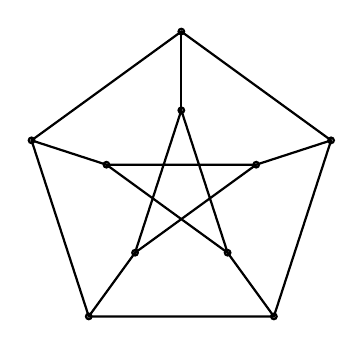
\begin{tikzpicture}[style=thick]
\draw (18:2cm) -- (90:2cm) -- (162:2cm) -- (234:2cm) --
(306:2cm) -- cycle;
\draw (18:1cm) -- (162:1cm) -- (306:1cm) -- (90:1cm) --
(234:1cm) -- cycle;
\foreach \x in {18,90,162,234,306}{
\draw (\x:1cm) -- (\x:2cm);
\draw (\x:2cm) circle (1pt);
\draw (\x:1cm) circle (1pt);
}
\end{tikzpicture}
{$G$}=Petersen graph
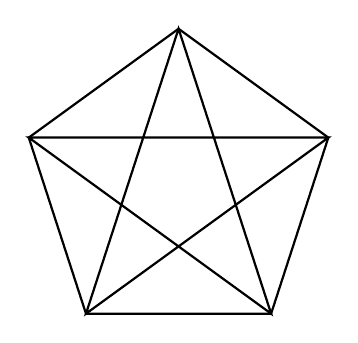
\begin{tikzpicture}[style=thick]
\draw (18:2cm) -- (90:2cm) -- (162:2cm) -- (234:2cm) --
(306:2cm) -- cycle;
\draw (18:2cm) -- (162:2cm) -- (306:2cm) -- (90:2cm) --
(234:2cm) -- cycle;
\foreach \x in {18,90,162,234,306}{}
\end{tikzpicture}
{$K_5$} minor
\end {example}
\begin {remark} If {$G$} is planar then {$G$} has no {$K_5$} or {$K_{3,3}$} subdivision/minor as subgraph
\end {remark}
$(a) \implies (b)$ , $(a) \implies (c)$ are easy implications
\begin {proof} An embedding of {$G$} would contain an embedding of {$K_5$} or {$K_{3,3}$}
\end {proof}
\bigskip
\begin {theorem} (The Four-Color Theorem)
Every planar graph is 4-colorable.
\end {theorem}
\bigskip
\textbf{\textit{Proof history}}
\begin {itemize}
\item 1800-1850 first mentioned
\item 1852 a student of De Morgan conjectured 4-colors are sufficient
\item Cayley popularized it a lot
\item 1879 Alfred Kempe published a proof
\item 1880 Tait had another proof
\item 1890 Heawood found an error in Kempe's proof (but proved the 5-color theorem), 
                  Petersen found an error in Tait's proof
\item 1960 Heesh found a method that could give a proof but involved analysing a huge number of cases
\item 1976 Appel, Haken analysed these cases with a computer ($\approx$ 2000 cases)
\item 1990 Robertson, Seymour and others gave a new computer-assisted proof ($\approx$ 600 cases)
\end {itemize}
\bigskip
\begin {definition} A face is any connected component of ${\rm I\!R^2}$  after removing the embedded graph.
\end {definition}
\begin {observation}\begin{minipage}[t]{\linewidth}
\begin {itemize}
\item There is exactly one unbounded face.
\item Each face is an open subset of ${\rm I\!R^2}$.
\end {itemize}
\end {minipage}
\end {observation}
\begin {observation}
A graph is planar if and only if it can be embedded in ${S^2}$ (the sphere).
Suppose {$G$} is embedded in ${S^2}$.Pick a point of ${S^2}$ not in the embedding.
Use the stereographic projection to map {$G$} onto ${\rm I\!R^2}$.
Note that in a spherical embedding each face is bounded and homeomorphic to an open disk.
\end {observation}
\bigskip
\bigskip
\begin {example} {$Q_3$} as planar graph.
\begin{tikzpicture}[style=thick]
\draw (0,0) -- (2,0) -- (2,2) -- (0,2) -- (0,0)
(0.5,0.5) -- (1.5,0.5) -- (1.5,1.5) -- (0.5,1.5) -- (0.5,0.5)
(0.5,0.5) -- (0,0)
(1.5,0.5) -- (2,0)
(1.5,1.5) -- (2,2)
(0.5,1.5) -- (0,2);
\end {tikzpicture}
\end {example}
\bigskip
\underline{\textbf{Notation}} Suppose I have {$G$} with a fixed planar embedding (or spherical embedding)
\newline
				     {$v$}= \# vertices, {$e$}= \# edges, {$f$}= \# faces.
\begin {theorem}
(Euler's formula) If G is planar and connected, then for any planar embedding of {$G$} :   
$$v-e+f=2.$$
\end {theorem}
\begin {proof}
By induction
\newline
If {$f$}={$1$} then {$G$} has no cycles, as otherwise any cycle of the graph would seperate ${\rm I\!R^2}$ into at $\geq 2$ parts. Hence {$G$} is a tree, $e=v-1$ and
$$v-e+f=v-(v-1)+1=2.$$
If $f\geqslant 2$ then pick an edge $xy\in E(G)$ so that on the two sides of {$xy$} we have two different faces of the embedding.
Now {$G-xy$} is planar, connected and it has 
{$f(G-xy)$}={$f(G)-1$},
{$e(G-xy)$}={$e(G)-1$},
{$v(G-xy)$}={$v(G)$}. 
The proof follows by induction.
\end {proof}
\bigskip
Euler cared about regular polyhedra in ${\rm I\!R^3}$
\newline
\underline{\textbf{Very quick application}}: Classification of Platonic solids (regular polytopes).
\begin {definition} A polytope is regular if:
\begin {enumerate}
\item All vertices have the same degree $k\geqslant3$,
\item All faces are polygons with the same number of sides $l\geqslant3$.
\end {enumerate}
\end {definition}
Let it have {$v$} vertices, {$e$} edges, {$f$} faces in the spherical embedding.

We have these equations:
$\begin{cases}
v-e+f=2\\
kv=2e \\
lf=2e 
\end {cases}$

and so:

$e(\frac{2}{k}-1+\frac{2}{l})=2 \implies \frac{2}{k}+\frac{2}{l}=1+\frac{2}{e}\implies \frac{1}{k}+\frac{1}{l}=\frac{1}{2}+\frac{2}{e}\textgreater \frac{1}{2}$. 

This can be satisfied only for $(k,l)=(3,3),(3,4),(3,5),(4,3),(5,3)$. For each case we uniquely determine $v,e,f$.

\begin{corollary}\begin{minipage}[t]{\linewidth}
Suppose $G$ has at least three vertices.
\begin {enumerate}[(a)]
\item If {$G$} is planar then $e\leqslant3v-6$
\item  If {$G$} is planar and triangle free then $e\leqslant2v-4$
\end {enumerate}
\end {minipage}
\end {corollary}
\begin {proof} We can assume {$G$} is connected. Then $v-e+f=2$.
Count the edges around each face. Each face has length $\geqslant3$ so we get at least ${3f}$.
But each edge is counted twice, so we get exactly $2e$. That means 
$2e\geqslant3f$ or $f\leqslant\frac{2}{3}e$.
\newline
$2=v-e+f\leqslant v-e+ \frac{2}{3}e=v- \frac{1}{3}e$
\newline
$e\leqslant 3v-6$
\newline
If {$G$} is triangle-free then we have a stronger inequality
$2e\geqslant 4f$
and continue the same way.
\end {proof}
\begin {observation} This gives another proof of non-planarity of {$K_{3,3}$} and {$K_5$}
\newline
{$K_5$}: $v=5,e=10$    \: \:\:\:\:\: $10\nleq3\cdot5-6$
\newline
{$K_{3,3}$}: is triangle-free, $v=6, e=9 \: \: \: \: 9\nleq2\cdot6-4$
\end {observation}





\begin{theorem}[5-color theorem]
If $G$ is planar then $\chi(G) \leq 5$.
\end{theorem}
\begin{proof}
Later: "Proof from the book" (Aigner, Zeigler).
\end{proof}

List coloring, examples:
\begin{itemize}
\item[1]A graph $G(V,E)$ with
	\begin{itemize}
	\item V = courses
	\item E = conflicts (student in both courses)
	\end{itemize}
	can be subject to a list-coloring should there restrictions to for instance  the choices of days that a course can be held at. 
\item[2]Soduku $\equiv$ coloring of $9\times 9$ grid with restrictions in the form of already given numbers.
\end{itemize}

As a definition:
\begin{definition}
Let $G$ be any graph, for every vertex $x\in V(G)$ we have a set of colors $L(x)$ ( of colors available to $x$).

A $L$-coloring of $G$ is a coloring $c:V(G)\rightarrow \underset{x}{\bigcup} L(x)$ such that $c(x)\in L(x)$ for all $x$. 

The list-chromatic number $\chi_{\ell}(G)$ is the smallest $k$ s.t. $G$ has a $L$-coloring for any choice of list satisfying $|L(x)|\geq k$. 

$G$ is $k$-list-colorable ($k$-choosable) when $\chi_{\ell}(G)\leq k$.
\end{definition}

\begin{example}
Here are some various examples and facts:

\begin{itemize}
\item $L(x)=\{1,\ldots,k\}$ for all $x\in V(G)$ then $L$-coloring $\equiv$ $k$-coloring in the normal sense
\item $\chi(G)\leq \chi_{\ell}(G)$
\item Example with $\chi(G) < \chi_{\ell}(G)$:
\begin{center}
\begin{tikzpicture}[
every node/.style={circle,inner sep=2pt,fill,draw}
]
\node[label={[label distance=1pt]90:$2,3$}] (A) at (-2,1) {};
\node[label={[label distance=1pt]90:$1,2$}] (B) at (0,1) {};
\node[label={[label distance=1pt]90:$1,3$}] (C) at (2,1) {};

\node[label={[label distance=1pt]270:$1,3$}] (D) at (-1,-1) {};
\node[label={[label distance=1pt]270:$1,2$}] (E) at (1,-1) {};
\node[label={[label distance=1pt]270:$2,3$}] (F) at (3,-1) {};

\draw[thick] (A) -- (D);
\draw[thick] (A) -- (E) ;

\draw[thick] (B) -- (D);
\draw[thick] (B) -- (F);
\draw[thick] (B) -- (E);

\draw[thick] (C) -- (E);
\draw[thick] (C) -- (F);

\end{tikzpicture}
\end{center}
For each $x$, $|L(x)|=2$. But for these list there are no $L$-coloring. Therefore $\chi_{\ell}(G)\geq 3$, while $\chi(G)=2$ since the graph is bipartite.
\item $\chi_{\ell}(G)\leq \Delta G+1$, same proof as the non-list chromatic number.
\item Brooks Theorem holds.
\end{itemize}
\end{example}

\textbf{Question:} Can we construct $G$ with small $\chi(G)$ and large $\chi_{\ell}(G)$?

\begin{proposition}
For every $k\geq 2$ there exist a graph with $\chi(G)=2$ and $\chi_{\ell}(G)>k$
\end{proposition}

\begin{proof}
Take $A=B=\binom{\{1,\ldots,2k-1\}}{k}$, (the set of all $k$-subsets of $\{1,\ldots,2k-1\}$).

Let $G=K_{A,B}$ be the complete bipartite graph with parts $A$ and $B$.
\begin{example}
Take $k=3, |A|=|B|=\binom{5}{3}=10$

That is $A$ and $B$ will consist of 10 vertices each with a list of three numbers made of the various permutations of $[1,2,3,4,5]$ and every vertex in $A$ is connected to every vertex in $B$. So $|V|=20, |E|=100$.
\end{example}

(\textit{proof} cont.)
For $X \in A$ or $X \in B$ set $L(X)=X$ and note $|L(X)|=k.$
We claim that $K_{A,B}$ has no $L$-coloring.

Suppose $c$ is an $L$-coloring. Then $c(A)\subseteq \{1,\ldots,2k-1\}$, $|c(A)|\geq k$. $\leftarrow$ will be true, or otherwise $|c(A)|\leq k-1$ and then there is a $X\subseteq\{1,\ldots,2k-1\}$ such that $|X|=k$ and $X\cap c(A)=\emptyset$. Then $X$ cannot be colored with a color from $L(X)$.

Similar for $B$, that is  $c(B)\subseteq \{1,\ldots,2k-1\}$, $|c(B)|\geq k$.

It follows  that $c(A)\cap c(B)\neq \emptyset$ so two vertices on opposite sides have the same color. That means $\chi_{\ell}(K_{A,B})\geq k+1$, but $\chi(K_{A,B})=2$.
\end{proof}

\begin{theorem}
(Thomassen 1994)

Every planar graph satisfies $\chi_{\ell}(G)\leq 5$. (It is 5-list-colorable).  
\end{theorem}
\begin{remark}
This is stronger than the 5-color theorem, because $\chi(G)\leq \chi_{\ell}(G)$.
\end{remark}

\begin{definition}
An embedding of a planar graph $G$ is called:
\begin{itemize}
\item A triangulation if every face is a triangle (also the unbounded one)
\item A near-triangulation if every bounded face is a triangle and the unbounded one is a cycle.
\end{itemize}
\end{definition}

\begin{example}
Various examples of Definition 8.
\begin{center}
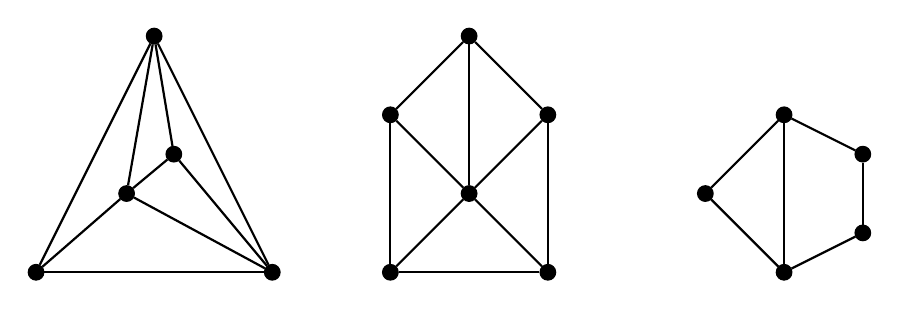
\begin{tikzpicture}[
every node/.style={circle,inner sep=2pt,fill,draw}
]
\node (a) at (-5,2) {};
\node (b) at (-5.35,0) {};
\node (c) at (-4.75,0.5) {};
\node (d) at (-6.5,-1) {};
\node (e) at (-3.5,-1) {};

\draw[thick] (a) -- (b);
\draw[thick] (a) -- (c) ;
\draw[thick] (a) -- (d);
\draw[thick] (a) -- (e);
\draw[thick] (b) -- (c);
\draw[thick] (b) -- (d);
\draw[thick] (b) -- (e);
\draw[thick] (d) -- (e);
\draw[thick] (c) -- (e);

\node (f) at (-2,-1) {};
\node (g) at (-2,1) {};
\node (h) at (-1,0) {};
\node (i) at (-1,2) {};
\node (j) at (0,-1) {};
\node (k) at (0,1) {};

\draw[thick] (f) -- (g);
\draw[thick] (g) -- (i);
\draw[thick] (i) -- (k);
\draw[thick] (j) -- (k);
\draw[thick] (j) -- (f);
\draw[thick] (h) -- (f);
\draw[thick] (h) -- (g);
\draw[thick] (h) -- (i);
\draw[thick] (h) -- (k);
\draw[thick] (h) -- (j);

\node (l) at (2,0) {};
\node (m) at (3,1) {};
\node (n) at (3,-1) {};
\node (o) at (4,0.5) {};
\node (p) at (4,-0.5) {};

\draw[thick] (l) -- (m);
\draw[thick] (m) -- (o);
\draw[thick] (o) -- (p);
\draw[thick] (p) -- (n);
\draw[thick] (n) -- (l);
\draw[thick] (n) -- (m);

\end{tikzpicture}
\end{center}
From left to right: A triangulation, a near triangulation and the final picture is neither.
\end{example}

\begin{remark}
Every embedding can be extended to a triangulation on the same vertex set. (By only adding edges)
\end{remark}
\begin{proof}
Add diagonals as needed. It also work for the unbounded face.
\end{proof} 

In other words:
For any planar $G$ there is a triangulation $H$ such that
\begin{align*}
V(G)=V(H), \ E(G)\subseteq E(H).
\end{align*} 
In particular
\begin{align*}
\chi(G) &\leq \chi(H)
\\
\chi_{\ell}(G) &\leq \chi_{\ell}(H)
\end{align*}

\begin{proposition}
Suppose $G$ is near-triangular with outer cycle $\mathbb{O}=x_1,\ldots,x_k$ and assume the following exist:
\begin{itemize}
\item $L(x_1)=\{a\}$, $L(x_2)=\{b\}$, $a\neq b$
\item $|L(x_i)|\geq 3$ for all $i=3,\ldots,k-1$
\item $|L(y)|\geq 5$ for all $y\notin \mathbb{O}$.
\end{itemize}
Then $G$ is L-colorable.
\end{proposition}

\begin{remark}
This proposition implies Thomassens theorem as follows:

Take $H$, any planar graph, with lists $L$ and $|L(x)| \geq 5$. Extend $H$ to a triangulation $H\subseteq G$ (in particular, $G$ is a near-triangulation). Choose any $x_1,x_2$ on the outer face. Restrict $L(x_1)$ and $L(x_2)$ to one element and voila! $\rightarrow$ the proposition applies to $G$. 

$L$-coloring of $G$ gives an $L$-coloring for $H$.
\end{remark}

\begin{proof}
Proof of proposition 11:

\begin{itemize}
\item $|V(G)|=3$: 
\begin{center}
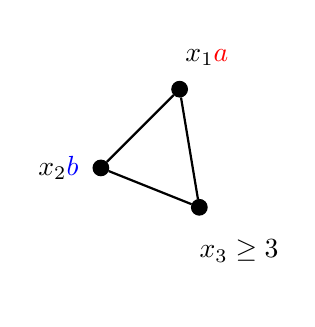
\begin{tikzpicture}[
every node/.style={circle,inner sep=2pt,fill,draw}
]
\node[label={[label distance=1pt]60:$x_1 {\color{red}a}$}] (A) at (1,1) {};
\node[label={[label distance=1pt]180:$x_2 {\color{blue}b}$}] (B) at (0,0) {};
\node[label={[label distance=1pt]300:$x_3 \geq 3$}] (C) at (1.25,-0.5) {};


\draw[thick] (A) -- (B);
\draw[thick] (A) -- (C) ;
\draw[thick] (B) -- (C);

\end{tikzpicture}
\end{center}
Then we will have a spare color for $x_3$.
\end{itemize}

\underline{Case 1}:

There is an edge $x_k x_j$, $j=2,\ldots,k-2$
\begin{center}
\includegraphics[scale=0.25]{Case1}
\end{center}
\begin{itemize}
\item[•]$G_1=$ graph bounded by $x_1x_2\ldots x_jx_k \rightarrow$ $L$-color $G_1$ by induction.
\item[•] $G_2=$ graph bounded by $x_kx_j\ldots x_{k-1} \rightarrow $ $L$-color $G_2$ by induction.
\item[•] $\rightarrow$ L-coloring of $G$. Note that after coloring $G_1$ some colors are not available for certain vertices of $G_2$, but there is enough left just to use the induction hypothesis for $G_2$.
\end{itemize}

\underline{Case 2}:

There are no edge $x_k x_j$, $j=2,\ldots,k-2$.
\begin{itemize}
\item Around $x_k$ we must have a sequence of triangles, since the interior is triangulated.
\item Let $N(X_k)=\{x_1,x_{k-1},y_1,\ldots,y_{\ell}\}$
\item Pick $c,d \in L(X_k)$, $c\neq d$, $c,d \neq a$.
\item Set $G'=G-x_k$ and note that $G' $ is a near-triangulation. 
\end{itemize}
\begin{center}
\includegraphics[scale=0.125]{Case2}
\end{center}
Consider the list:
\begin{align*}
L'(y_i)=L(y_i)\backslash \{c,d\} \ , \ L'(x)=L(x) \ \text{for any other} \ x \in G'
\end{align*}
$\leadsto$ There is a L'-coloring of $G'$ by induction.
\begin{align*}
c(y_i)\notin \{c,d\} \ , \ c(x_1) \notin \{c,d\}
\end{align*}
$\leadsto$ color $x_k$ with either $c$ or $d$ depending on $c(x_{k-1})$.
\end{proof}

\begin{remark}
There are planar not-4-list-colorable graphs. (Voigt '93 example with $\approx$ 300 vertices).
\end{remark}
\begin{remark}
Did not use Euler, upper/lower bounds. Only geometric properties.
\end{remark}
\subsubsection*{Application:
\underline{The art gallery problem}}

Suppose $P$ is a polygon in $\mathbb{R}^2$ with $n$ vertices.

\begin{example}
:
\begin{center}
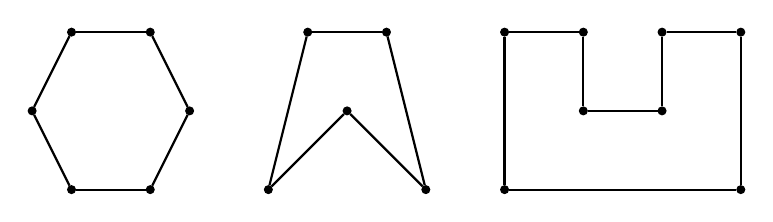
\begin{tikzpicture}[
every node/.style={circle,inner sep=1pt,fill,draw}
]
\node (a) at (-4,0) {};
\node (b) at (-3.5,1) {};
\node (c) at (-3.5,-1) {};
\node (d) at (-2.5,1) {};
\node (e) at (-2.5,-1) {};
\node (f) at (-2,0) {};

\draw[thick] (a) -- (b);
\draw[thick] (a) -- (c) ;
\draw[thick] (b) -- (d);
\draw[thick] (d) -- (f);
\draw[thick] (e) -- (f);
\draw[thick] (e) -- (c);

\node (g) at (-1,-1) {};
\node (h) at (-0.5,1) {};
\node (i) at (0,0) {};
\node (j) at (0.5,1) {};
\node (k) at (1,-1) {};

\draw[thick] (h) -- (g);
\draw[thick] (g) -- (i);
\draw[thick] (h) -- (j);
\draw[thick] (j) -- (k);
\draw[thick] (k) -- (i);

\node (l) at (2,-1) {};
\node (m) at (2,1) {};
\node (o) at (3,1) {};
\node (p) at (3,0) {};
\node (q) at (4,0) {};
\node (r) at (4,1) {};
\node (s) at (5,1) {};
\node (t) at (5,-1) {};

\draw[thick] (l) -- (m);
\draw[thick] (m) -- (o);
\draw[thick] (o) -- (p);
\draw[thick] (p) -- (q);
\draw[thick] (q) -- (r);
\draw[thick] (r) -- (s);
\draw[thick] (s) -- (t);
\draw[thick] (t) -- (l);


\end{tikzpicture}
\end{center}

\end{example}

We assume the bounded region is the floor plan af an art gallery.
\begin{quote}
How many guards are needed to guard each point in sight?
\end{quote}

\begin{problem}
\begin{itemize}
\item Find a gallery with 6 vertices requiring $\geq 2$ guards.
\item Find a gallery with as few vertices as possible requiring $\geq k$ guards.
\end{itemize}
\end{problem}

\begin{observation}
There are $n$-vertex galleries requiring at least $\left \lfloor \frac{n}{3} \right \rfloor$ guards.
\end{observation}
\begin{center}
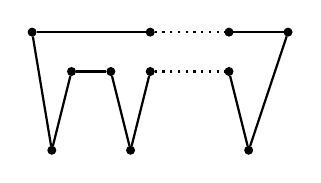
\begin{tikzpicture}[
every node/.style={circle,inner sep=1pt,fill,draw}
]
\node (a) at (-3.5,1.5) {};
\node (b) at (-3.25,0) {};
\node (c) at (-3,1) {};
\node (d) at (-2.5,1) {};
\node (e) at (-2.25,0) {};
\node (f) at (-2,1) {};
\node (g) at (-1,1) {};
\node (h) at (-0.75,0) {};
\node (i) at (-0.25,1.5) {};
\node (f') at (-2,1.5) {};
\node (g') at (-1,1.5) {};

\draw[thick] (a) -- (b);
\draw[thick] (b) -- (c) ;
\draw[thick] (c) -- (d);
\draw[thick] (d) -- (e);
\draw[thick] (e) -- (f);
\draw[dotted, thick] (f) -- (g);
\draw[thick] (g) -- (h);
\draw[thick] (h) -- (i);
\draw[dotted, thick] (f') -- (g');
\draw[thick] (i) -- (g');
\draw[thick] (a) -- (f');

\end{tikzpicture}
\end{center}

\begin{theorem}
Rephrasing the art gallery problem:

Every n-vertex gallery can be guarded by $\left \lfloor \frac{n}{3} \right \rfloor$ guards. ($\approx$ 70's Chvatal).
\end{theorem}

\begin{definition}
A planar embedding is called a \emph{polygon triangulation} if it is a near-triangulation and all vertices lie on the outer cycle.
\end{definition}

\begin{example}
"Polygon triangulated by diagonals"
\begin{center}
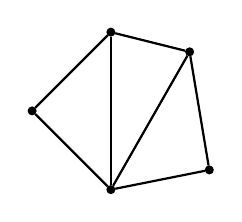
\begin{tikzpicture}[
every node/.style={circle,inner sep=1pt,fill,draw}
]
\node (a) at (-1,0) {};
\node (b) at (0,1) {};
\node (c) at (0,-1) {};
\node (d) at (1,0.75) {};
\node (e) at (1.25,-0.75) {};

\draw[thick] (a) -- (b);
\draw[thick] (a) -- (c);
\draw[thick] (c) -- (b);
\draw[thick] (d) -- (c);
\draw[thick] (b) -- (d);
\draw[thick] (c) -- (e);
\draw[thick] (d) -- (e);

\end{tikzpicture}
\end{center}
\end{example}

\begin{observation}
A triangulated polygon with n vertices has $2n-3$ edges, $n$ on the outer cycle and $n-3$ diagonals.
\end{observation}

\begin{observation}
Every triangulated polygon have a vertex of degree 2.
\end{observation}
\begin{proof}
The shortest diagonal cuts off such a vertex.
\end{proof}

\begin{observation}
Every triangulated polygon is 3-colorable.
\end{observation}
\begin{proof}
Take $v$ to be a vertex of degree 2. $G-v$ is a triangulated polygon. Color $G-v$ with 3 colors, the neighbours of $v$ will use 2 colors. Color $v$ with the spare color.
\end{proof}

\begin{proof}
Proof of Theorem 18:

\begin{itemize}
\item Let $G$ be planar polygon with $n$ vertices.
\item First triangulate using diagonals (Exercise: show that this is always possible).
\item The resulting triangular polygon is 3-colorable. 
\item Some color class will have $\leq \left \lfloor \frac{n}{3} \right \rfloor$ elements
\item Place guards at the vertices of that color.
\end{itemize}
\end{proof}
%%%%%%%%%%%%%%%%%%%%%%%%%%%%%%%%%%%%%%%%

\chapter{Chromatic polynomial}

Roughly lec7.tex, lec8.tex
\chapter{Edge coloring}

\section{Definitions and examples}

Until now we concentrated on coloring vertices of graphs. In this chapter we briefly address the concept of edge-coloring.

\begin{definition}
An \emph{edge-coloring} of $G=(V,E)$ is a function $f:E\rightarrow C$ (for some set of colors $C$) such that if two edges $e_1$, $e_2$ have a common endpoint then $f(e_1)\neq f(e_2)$. The \emph{edge chromatic number} (\emph{chromatic index}) $\chi'(G)$ is the smallest $k$ such that $G$ has an edge-coloring with colors $\{1,\dots,k\}$.
\end{definition}

[FIGURE]

\begin{example}[Cycles]
The $n$-cycle $C_n$ can be edge-colored with $2$ colors when $n$ is even and requires $3$ colors when $n$ is odd, therefore
$$\chi'(C_n)=
\begin {cases}
2 & 2|n\\
3 & 2\not|n
\end {cases}$$
\end{example}

\begin{example}[Scheduling]
Let $G$ be a bipartite graph whose two parts are $Classes$ and $Teachers$. There is an edge $tc$ if teacher $t$ is supposed to teach class $c$. How many time slots do we need to allocate to schedule all lessons?

[FIGURE]

The answer is $\chi'(G)$. Each color represents one time slot, and the edge-coloring condition guarantees that no teacher and no class is required to show up at two different events at the same time.
\end{example}

\begin{example}[Complete graphs]
As we all know a full soccer season in a league with $2k$ teams consists of $2k-1$ rounds. Each team plays exactly once in each round, and each pair meets once. This is just the statement that
$$\chi'(K_{2k})=2k-1.$$
Indeed, each color represents one week of the season, and the edges of a particular color determine the pairs of teams playing that week. We can of course make a more general statement about the edge-chromatic numbers of complete graphs:
$$\chi'(K_n)=
\begin {cases}
n-1 & 2|n\\
n & 2\not|n
\end {cases}$$
[FIGURE]

It is not hard to find a coloring. It $n=2k-1$ is odd, arrange the vertices into a regular $n$-gon. Choose a color class consisting of $k$ parallel edges (one vertex is left out). This color class has $n$ possible rotations. These rotations cover all edges of $K_n$. This is an edge-coloring with $n$ colors,so $\chi'(K_n) \leq n$. For an upper bound, take any edge-coloring of $K_n$. The color class $1$ must miss some vertex $v$. Since all edges incident to $v$ require $n-1$ colors, we get at least $1+(n-1)=n$ colors in total.

If $n=2k$ is even arrange $n-1$ vertices in a regular $(n-1)$-gon and place one vertex at the origin. Use $k-1$ parallel edges and one edge from the origin to the vertex on the perimeter being left out. This is one color class, and the $n-1$ rotations of this class form a desired edge-coloring. The upper bound is obvious.
\end{example}

\begin{lemma} 
$\chi'(G) \geq \Delta(G)$
\end{lemma}
\begin{proof}
We need at least $\Delta(G)$ colors just to color the edges incident to the vertex of maximum degree.
\end{proof}


\section{Basic properties}

As with vertex-colorings, also edge-colorings can be expressed using other familiar language of graph theory. In fact edge-colorings can be seen as a special case of vertex-colorings.

\begin{definition}
A \emph{matching} in $G$ is a set of edges, no two of which have a common endpoint.
\end{definition} 

This is a very important concept in graph theory. Equivalently, a matching in $G$ is a $1$-regular subgraph of $G$. 

\begin{proposition}
Let $G=(V,E)$ be a graph.
\begin{itemize}
\item If $f$ is an edge-coloring of $G$ then every color class $f^{-1}(c)$ is a matching.
\item An edge-coloring with $k$ colors is the same as a partition of $E$ into $k$ matchings.
\item For any two colors $c_1,c_2\in C$, $c_1\neq c_2$, the edge set $f^{-1}(c_1)\cup f^{-1}(c_2)$ is a disjoint union of cycles and paths.
\end{itemize}
\end{proposition}
\begin{proof}
The first two parts are clear. For the last one, note that in $f^{-1}(c_1)\cup f^{-1}(c_2)$ every vertex is of degree at most $2$.
\end{proof}

\begin{definition}
Let $G=(V,E)$. The \emph{line graph} $L(G)$ has vertex set $E$, and $e_1$, $e_2$ are adjacent in $L(G)$ if they share a common vertex in $G$.
\end{definition}

\begin{example}
The line graph simply keeps track of the incidence relation between the edges of $G$. 

[FIGURE]
\end{example}

All the entries in the following glossary should now be completely obvious. It translates edge-coloring notions into their vertex-coloring counterparts.

\begin{center}
\begin{tabular}{l|l}
Edges of $G$ & Vertices of $L(G)$ \\
\hline
{edge in $G$} & {vertex of $L(G)$} \\
{matching in $G$} & {independent set in $L(G)$} \\
{edge-coloring of $G$} & {vertex coloring of $L(G)$} \\
{$\chi'(G)$} &  {$\chi(L(G))$} 
\end{tabular}
\end{center}

We have $\omega(L(G))\geq \Delta(G)$ because all edges incident to a fixed vertex $v$ induce a clique in $L(G)$. That implies $\chi'(G)=\chi(L(G))\geq \omega(L(G))\geq \Delta(G)$ which we already knew. Moreover $\Delta(L(G))= \max_{uv\in E(G)}(deg_G(u)+deg_G(v)-2)\leq 2\Delta(G)-2$, so $\chi'(G)=\chi(L(G)) \leq \Delta(L(G))+1\leq 2\Delta(G)-1$. Altogether this shows
$$\Delta(G)\leq \chi'(G) \leq 2\Delta(G)-1.$$
In fact the situation is much ``better'', in that the uncertainty interval for $\chi'(G)$ is as short as possible without being trivial. There are only two possibilities for $\chi'(G)$\ !
\begin{theorem}
\label{thm:vizing}
(Vizing '64) For any graph $G$ we have
$$\Delta(G)\leq \chi'(G) \leq \Delta(G)+1.$$
\end{theorem}
\begin{remark}
In some older literature graphs with $\chi'(G)=\Delta(G)$ are called ``Class 1'' and those with $\chi'(G)=\Delta(G)+1$ are called ``Class 2''. (Un?)surprisingly it is still NP-hard to recognize if $\chi'(G)=\Delta(G)$ or $\chi'(G)=\Delta(G)+1$, even for graphs with $\Delta(G)=3$.
\end{remark}

In the next section we will prove that bipartite graphs are Class 1. The main tool is one of the most classical results in combinatorics --- Hall's marriage theorem, which we discuss next.


\section{Hall's marriage theorem and applications}

Here is a version of the question commonly known as \emph{Hall's marriage problem}, first studied by Hall in the 1930s. We have a number of boys and girls, and each girl fancies some of the boys. We want to pair them up so that each girl is in a couple with a boy she fancies. Under what conditions is such a pairing possible?\footnote{As dictated by the political correctness of the 21st century, we ignore the preferences of the boys and we let some of the boys to leave without a girl.}

There are obvious necessary conditions that must be met for this to work. For example, each girl must fancy at least one boy. Of course this is not enough, because two girls might desire only one and the same boy. We can avoid this situation with a more general necessary condition: every set of $k$ different girls must altogether like at least $k$ different boys, for each $k\geq 1$. Hall's marriage theorem states that this necessary condition is also sufficient. Here it is in the language of bipartite graphs.

\begin{theorem}
(Hall 1935) Suppose $G$ is a bipartite graph with parts $V(G)=A\cup B$, such that for every $X\subseteq A$ we have:
$$|\bigcup_{x\in X}N_G(x)|\geq |X|.$$
Then $G$ has a matching of size $|A|$.
\end{theorem}
\begin{proof}
Write $N_G(X)=\bigcup_{x\in X} N_G(x)$ and let $n=|A|$. The proof is by induction on $n$. If $n=0$ there is clearly nothing to do. Otherwise we split the proof into two cases.

\begin{itemize}
	\item Suppose that for any $\emptyset\neq X\subsetneq A$, $|N_G(X)|\geq|X|+1$, so the inequality always holds with a surplus. Take any $a\in A$, $b\in N_G(a)$, match them, and use the inductive assumption in the graph $G'=G[A-a,B-b]$. This is possible because for any $X'\subseteq A-a$ we have $|N_{G'}(X)|\geq |N_G(X)|-1 \geq (|X|+1)-1=|X|$.

	\item Now suppose there is a set $\emptyset\neq X\subsetneq A$ with $N_G(X)=|X|$. Then by induction we find appropriate matchings in $G'=G[X,N(X)]$ and $G''=G[A-X,B-N(X)]$ and join them to form a matching in $G$. The only nontrivial fact to be checked is that $G''$ satisfies the inductive assumption. Pick any $Y\subseteq A-X$. Then $$|Y|+|X|=|Y\cup X|\leq|N_G(Y\cup X)|=|N_G(X)|+|N_G(Y)\cap(B-N(X))|=|X|+|N_G(Y)\cap(B-N(X))|.$$ 	It follows that $|Y|\leq |N_G(Y)\cap(B-N(X))| = |N_{G''}(Y)|$ as required.
\end{itemize}
[FIGURES]
\end{proof}

The marriage theorem has many interesting applications, especially to regular configurations, often combined with a counting argument as below.

\begin{example}
Split the standard 52 card deck into 13 piles of 4 cards each. Regardless of the splitting we can choose 1 card from each pile, so that we have one card of each rank: $A,2,3,\dots,K$.

To see this, construct a bipartite graph $G$ where the two parts are $R$ (ranks) and $P$ (piles). There is an edge $rp\in E(G)$ if pile $p$ contains a card of rank $r$. A matching in $G$ with 13 edges determines a bijection $P\longleftrightarrow R$. All we need to do is find such a matching with Hall's theorem.

[FIGURE]

Take any subset $X\subseteq R$ of ranks. This subset represents $4\cdot|X|$ actual cards. Since each plie has size 4, these $4|X|$ cards must occupy at least $|X|$ piles. But that means that the ranks in $X$ are adjacent to at least $|X|$ piles in $|P|$ in total, which is exactly the statement $|N_G(X)|\geq|X|$.
\end{example}

Note that in the above example cards of one rank (say all aces) can be distributed to less than 4 piles, so it would be more convenient to represent the situation with a \emph{multigraph}, where multiple edges between vertices are allowed.

[FIGURE]

This is the only part of these notes where we use the concept of a multigraph. Without going into too much formalism let us just note that the multiple edges adjacent to a vertex all contribute to its degree, so in the example above each vertex in $R$ has degree 13 and each vertex in $P$ has degree $4$ (in the multigraph sense).

Repeating a very similar argument yields the next theorem.

\begin{theorem}
\label{thm:chip-d-regular}
If $G=(V,E)$ is a $d$-regular bipartite multigraph, then $\chi'(G)=d$.
\end{theorem}
\begin{proof}
Denote by $V=A\cup B$ the parts of the bipartition. Then $|A|=|B|=n$, because $d\cdot |A|=|E|=d\cdot |B|$. 

We prove the theorem by induction. If $d=1$ then $G$ itself is a matching, so we are done. Let $d\geq 2$. We will first use Hall's theorem to show the existence of a matching of size $n$ in $G$. Take any $X\subseteq A$ and let $e_X$ be the number of edges in $G[X,N_G(X)]$. Then $d\cdot |X|=e_X\leq d\cdot |N_G(X)|$, so $|X|\leq |N_G(X)|$. From Hall's theorem, we get a matching $M$ of size $n$ in $G$. Since $G-M$ is a $(d-1)$-regular multigraph, by induction $\chi'(G)\leq 1 + (d-1) = d$.
\end{proof}

\begin{remark}
If $G$ is a bipartite miltigraph with both parts of size $n$ then a matching of size $n$ is called a \emph{perfect matching}.
\end{remark}

We can now prove that all bipartite graphs are of Class 1.

\begin{theorem}(K\"onig)
If $G=(V,E)$ is a bipartite multigraph, then $\chi'(G)=\Delta (G)$.
\end{theorem}

\begin{proof}
Let $V=A\cup B$ be the two parts. We can assume $|A|=|B|=n$. (If not, then add extra isolated vertices to the smaller part). Write $\Delta := \Delta(G)$. If $A$ has a vertex $v$ of degree less than $\Delta$, then $|E|<\Delta n$, therefore also $B$ has some vertex of degree less than $\Delta$, call it $u$. In this case add a new edge $uv$ to the multigraph. Repeat this process until the graph is $\Delta$-regular. By Theorem~\ref{thm:chip-d-regular} we get that the expanded graph (and even more so its original subgraph) is $\Delta$-edge-colorable.
\end{proof}



\section{Edge coloring vs. the 4-color theorem.}

With every planar triangulation (that is, a planar graph embedded so that all faces are triangles), we can associate a dual planar graph. This classical construction has tremendous applications in the theory of planar graphs. (In fact the dual graph can be defined for any planar graph, not necessarily a triangulation, but we will not require that generality).

[FIGURE]

Let $G=(V,E)$ be a planar graph together with a planar embedding such that every face (including the unbounded one) is a triangle. We denote the set of faces of the embedding by $F(G)$.

\begin{definition}
The dual graph $G^*$ of $G$ is defined by the conditions: $V(G^*)=F(G)$ and $f_1f_2\in E(G^*)$ if $f_1,f_2$ are two faces of $G$ that share a common edge. 
\end{definition}

It is helpful to represent each vertex of $G^*$ as a point inside the corresponding face.

[FIGURE]

\begin{observation}
By construction $G^*$ has the following properties:
\begin{itemize}
    \item $G^*$ is 3-regular. (Since every face has 3 neighbours along common edge.)
    \item $|E(G^*)|=|E(G)|.$ (The bijection is determined by the ``crossing'' relation.)
    \item $G^*$ is planar.
    \item Every face of $G^*$ contains exactly one vertex of $G$.
    \item $|V(G^*)|=|F(G)|$, $|E(G^*)|=|E(G)|$,  $|F(G^*)|=|V(G)|$.
\end{itemize}
\end{observation}

We introduced this concept because of a beautiful relation between vertex $4$-colorings of $G$ and edge $3$-colorings of its dual $G^*$. This was, in fact, what Tait showed in his incomplete proof of the $4$-colour theorem in 1878. 

\begin{theorem}[Tait 1878]
Suppose $G$ is a planar triangulation. TFAE:
\begin{enumerate}
    \item[a)] $G$ is vertex $4$-colorable.
    \item[b)] $G^*$ is edge $3$-colorable.
\end{enumerate}
\end{theorem}

\begin{proof}
\emph{a) $\Rightarrow$ b).} Take a 4-coloring $c:V(G)\rightarrow \{00,01,10,11\}$. We will construct an edge coloring of $G^*$ a follows: if $e^*$ is the dual edge of an edge $e=xy$, then we set

$$f(e^*)=c(x)\oplus c(y),$$

where $\oplus$ denotes XOR --- coordinate bitwise exclusive OR.

[FIGURE]
    
Let's check that $f$ is an edge 3-coloring.
\begin{itemize}
    \item $f(e^*)\neq 00$ because $c(x)\neq c(y)$, therefore $im(f)	\subseteq\{01,10,11\}$.
    \item Take $e_1^*,e_2^*\in E(G^*)$ sharing a common vertex in $G^*$ as in the figure. We must have $e_1=xy$ and $e_2=yz$ for some triangle $xyz$ in $G$. Then $f(e_1^*)\oplus f(e_2^*)=c(x)\oplus c(y) \oplus c(y)\oplus c(z)=c(x)\oplus c(z) \neq 00$, because $c(x)\neq c(z)$.

        [FIGURE]
\end{itemize}

\smallskip    
\emph{b) $\Rightarrow$ a).} Start with an edge 3-coloring $f:E(G^*)\rightarrow \{1,2,3\}$. Since $G^*$ is $3$-regular, every color appears at every vertex of $G^*$. For $i=1,2$ let $H_i \subseteq G^*$ be the subgraph spanned by the edge set $f^{-1}(i)\cup f^{-1}(3)$.
  
[FIGURE]

Each $H_i$ is 2-regular, hence it is a union of cycles. Construct a coloring $c:V(G)\rightarrow \{00,01,10,11\}$ using the following definition. For a vertex $v\in V(G)$ and for $i=1,2$, the $i$-th bit of $c(v)$ is \begin{center}\emph{the parity of the number of cycles in $H_i$ which contain $v$ inside}\end{center}.

[FIGURE-EXAMPLE]

Note that each $H-i$ is just a simple polygon in $\mathbb{R}^2$ and $v$ is inside a polygon if a generic ray from $v$ intersects the polygon an odd number of times. With this observation we can prove that $c$ is a vertex-coloring of $G$. Take an edge $e=uv\in E(G)$. We want to show $c(u)\neq c(v)$. 

[FIGURE]

W.l.o.g. suppose that $f(e^*)=1$. Then the dual edge $e^*$, which belongs to some cycle $C$ of $H_1$, intuitively ``separates'' $u$ and $v$. More precisely, counting the intersections between generic rays from $u$ and $v$ with $H_1$ we prove the following two claims:

\begin{itemize}
    \item $v$ and $u$ are on the opposite sides of $C$,
    \item for any other cycle of $H_1$, both $u,v$ are inside or both $u,v$ are outside that cycle.
\end{itemize}
As a consequence $c(v)$ and $c(u)$ differ at position $i=1$. The proof when $f(e^*)=2$ and $f(e^*)=3$ is similar. That shows $c$ is a vertex coloring.
\end{proof}



\section{Exercises}

\begin{enumerate}
\item Prove: if $G$ is connected and $L(G)$ is isomorphic to $G$ then $G$ is a cycle.
\item Suppose that $G$ has $n$ vertices and $m$ edges. Show that $\chi'(G)\geq m/\lfloor n/2\rfloor$. Use it to show that the $5$-vertex graph below is of Class 2, and to reprove that $\chi'(K_{2k-1})=2k-1$. [FIGURE]
\item We observed that $\omega(L(G))\geq\Delta(G)$. Find an exact formula for $\omega(L(G))$.
\item Suppose $G$ is $r$-regular with an odd number of vertices. Prove that $r$ is even and that $\chi'(G)=r+1$.
\item Find the edge-chromatic number of the Petersen graph.
\end{enumerate}

\chapter{Chromatic number of Euclidean spaces}

Roughly lec11.tex, lec12.tex, lec13.tex
\chapter{Coloring and topology}


\section{Exercises}

\begin{enumerate}
\item Can the directed graph formed in the proof of oriented Sperner's lemma really have cycles, or is it just a union of directed paths?

\item Prove that Sperner's lemma and Brouwer's fixed point theorem are equivalent in the following sense: Find a proof of the ``classical'' version of Sperner's lemma from Brouwer's theorem.

\smallskip
Hint: Construct a continuous map $f:\Delta\to \Delta$ by defining it on the vertices of the triangulation and extending linearly to the interiors of the edges and triangles of the triangulation. Arrange it so that any fixed point of $f$ must lie inside a $3$-colored triangle.

\item Use Sperner's lemma to prove the following classical fact about rectangle dissections:

Suppose a rectangle is partitioned into smaller rectangles, and that each small rectangle has at least one side of integer length. Prove that the big rectangle also has at least one side of integer length.

\smallskip
Hint: Subdivide each small rectangle with one diagonal to get a triangulation of the big rectangle. Place everything in a coordinate system with one corner at $(0,0)$. Color each vertex $P=(x,y)$ with 
\begin{itemize}
\item color $1$ if $x\in\ZZ$,
\item color $2$ if $x\not\in\ZZ$ and $y\in \ZZ$,
\item color $3$ if $x,y\not\in\ZZ$.
\end{itemize}
Prove that there is no triangle with colors $1,2,3$. Finally show that assuming both sides of the big rectangle are non-integers contradicts Sperner's lemma.
\end{enumerate}
\chapter{Exam problems}

To be written, MA

%------------------------
\begin{thebibliography}{99}
\bibitem[D]{diestel} R. Diestel, Graph Theory, Graduate Texts in Mathematics 173, Springer--Verlag  
\end{thebibliography}

\end{document}

%-----------------------

